% -*-coding: utf-8 -*-
% Держать в начале каждого файла!

\documentclass[a4paper, 12pt]{extarticle}
\usepackage{metod}

\MTDSetPhysSection{Механика}
\MTDSetTitle{Измерение ускорения свободного падения с~помощью математического маятника}
\MTDDesignator{М--11}
\MTDSetGrade{10}

\MTDSetAuthors{И.~Н.~Грачева, В.~И.~Гребенкин, А.~Е.~Иванов, И.~А.~Коротова,
Е.~И.~Красавина, А.~В.~Кравцов, Н.~С.~Кулеба, Б.~В.~Падалкин,
Г.~Ю.~Шевцова, Т.~С.~Цвецинская}

\MTDSetEditorsGenCase{И.~Н.~Грачевой, А.~Е.~Иванова, А.~В.~Кравцова}

\newcommand{\eps}{\epsilon}
\newcommand{\isum}{\sum\limits_{i=1}^{n}}


\begin{document}

\MTDTitlePage
\MTDInfoPage

\setcounter{section}{11}

\subsection{Цель работы}
Определение значения ускорения свободного падения и экспериментальная проверка закономерностей движения математического маятника. 

\subsection{Основные теоретические сведения}

\begin{wrapfigure}{r}{0.22\textwidth}
 \centering
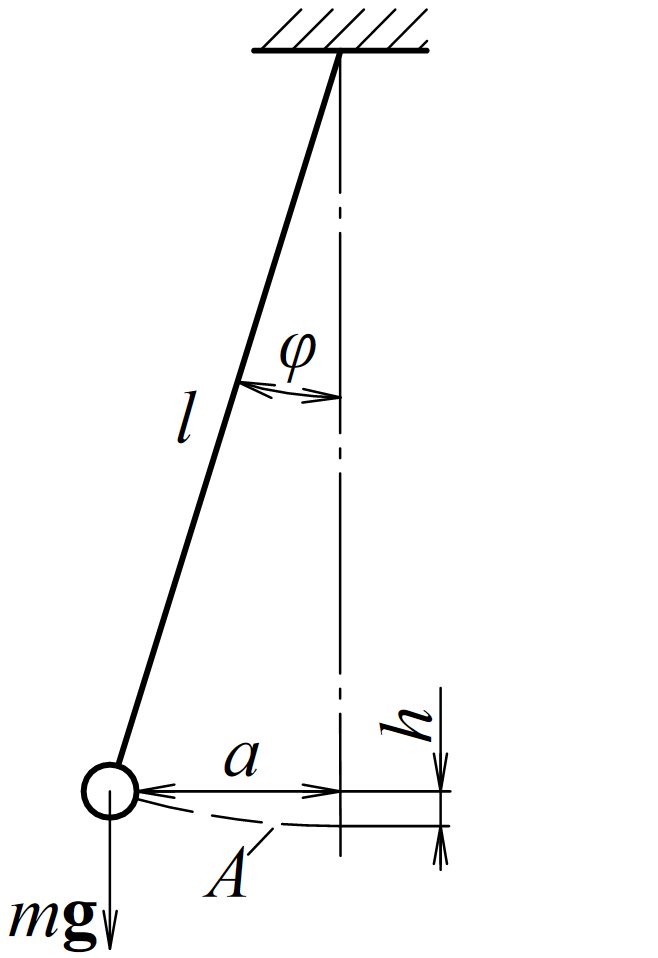
\includegraphics[width = 0.93\linewidth, keepaspectratio=true]{M11-PendledumOscillator}
\caption{\label{fig:m11-pendulum}}
\end{wrapfigure}

В физике под маятником понимают твёрдое тело, совершающее под действием силы тяжести колебания вокруг неподвижной точки или оси. 

Математическим маятником называют идеализированную систему, состоящую из невесомой нерастяжимой нити, на которой подвешена масса, сосредоточенная в одной точке. Достаточно хорошим приближением к математическому маятнику служит небольшой тяжёлый шарик, подвешенный на длинной тонкой нити. Отклонение маятника от положения равновесия будем характеризовать углом $\varphi$, образованным нитью и вертикалью (рис.~\ref{fig:m11-pendulum}). % ИЗМ: "хорошем" -> "хорошим"; нитью С вертикалью -> нитью И вертикалью

Будем рассматривать малые колебания, когда угол $\varphi$ не превосходит нескольких градусов. В этом случае $\sin \varphi \approx \varphi$, а дуга $A$ и хорда $a$ практически совпадают, так что в первом приближении можно считать движение груза прямолинейным, а колебания "--- гармоническими (происходящими по гармоническому закону синуса или косинуса). Таким образом, при малых амплитудах математический маятник совершает гармонические колебания с частотой~$\omega_0 = \sqrt{\frac{g}{l}}$ и периодом~$T = 2 \pi \sqrt{\frac{l}{g}}$. %ИЗМ: происходящЕЙ -> происходящими | мб вынести формулы или dfrac | больше никаких \ell, так как нигде в методичке они больше не встречаются

Формулой периода можно воспользоваться для определения ускорения силы тяжести в той или иной точке Земли, поскольку длину маятника и период его колебаний можно измерить весьма точно. 
%зачем этот новый абзац?

Ускорение свободного падения в разных точках Земли несколько различно. При не очень точных измерениях этой разницей (которая не превышает 0,6\%) пренебрегают и считают $g = 9,81~\Units{\text{м}/\text{с}^2}$. 

\subsection{Описание экспериментальной установки}
Схема установки показана на рис.~\ref{fig:m11-equipment}. В качестве математического маятника используется металлический шар~\emph{3}, подвешенный на двух капроновых нитях к кронштейну~\emph{2}. На этом же кронштейне укреплён фотодатчик~\emph{4}. Расстояние между кронштейнами определяется по нанесённой на штатив шкале~\emph{5}. 

\begin{figure}[h] % никак она тут не встанет; линии нитей превратились в ужас
\begin{center}
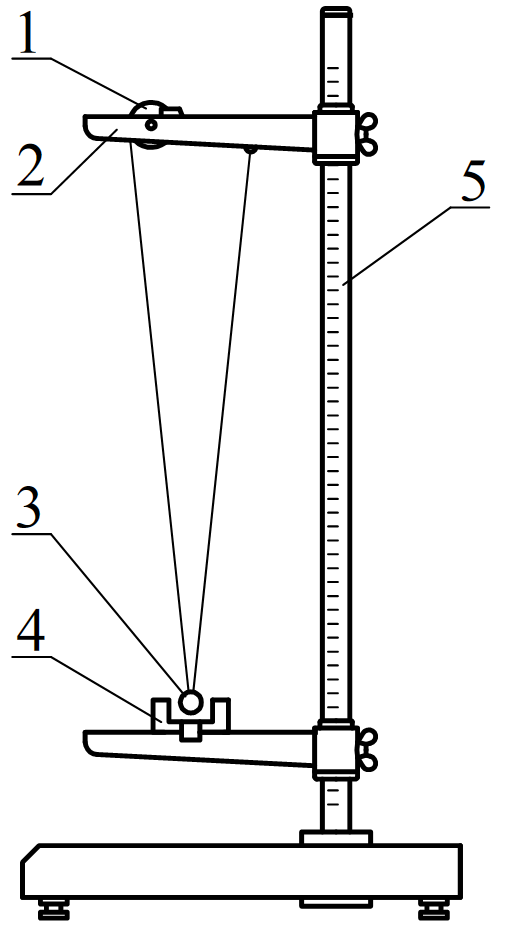
\includegraphics[width = 0.25\linewidth, keepaspectratio=true]{M11-PendledumOscillatorMachine}
\end{center}
\caption{Схема установки \label{fig:m11-equipment}}
\end{figure}

\subsection{Порядок выполнения эксперимента}
\begin{enumerate}
\item Установите нижний кронштейн с фотодатчиком~\emph{4} в крайнее нижнее положение шкалы~\emph{5} так, чтобы верхняя плоскость кронштейна совпала с одной из рисок шкалы. Установите верхний кронштейн таким образом, чтобы шарик~\emph{3} математического маятника оказался в рабочей зоне фотодатчика. Вращая  ролик~\emph{1}, добейтесь такого положения шарика, при котором его центральная риска будет совпадать по высоте с риской на     фотодатчике. По шкале на вертикальной стойке определите длину математического маятника~$l_1$.
\item Приведите математический маятник в колебательное движение, отклонив металлический шарик на угол 5--6\degree, после чего нажмите на кнопку <<СБРОС>> на блоке. По показанию таймера определите значение времени 40--50 колебаний маятника. Определите среднее значение периода колебания маятника по формуле $T_1 = t_1 / N$, где $t_1$ "--- время колебаний, $N$ "--- число колебаний. %ИЗМ: "градусов" заменила на \degree | 40...50 на 40--50 заменила | мб формулу вынести | неужели "сброс" - это именно та кнопка, которую стоит нажимать?
\item Передвиньте вверх кронштейн с фотодатчиком на два деления шкалы вертикальной стойки. Вращая ролик~\emph{1}, добейтесь такого положения шарика, при котором его центральная риска будет совпадать по высоте с риской  на фотодатчике. По шкале вертикальной стойки определите длину математического маятника $l_2$. Повторите эксперимент по п.~2. 
\item Повторите эксперимент по п.~3, уменьшая длину маятника, 6~раз, запишите  полученные результаты в таблицу~\ref{tab:m11-res-exp}. %6 раз наверное до дееприч. оборота

\begin{table}[h]
\caption{\label{tab:m11-res-exp}}
\begin{flushright}
\begin{tabular}{|c|>{\centering\arraybackslash} m{1.4cm}|>{\centering\arraybackslash} m{0.85cm}|>{\centering\arraybackslash} m{0.85cm}|>{\centering\arraybackslash} m{0.85cm}|>{\centering\arraybackslash} m{1.4cm}|>{\centering\arraybackslash} m{1.4cm}|>{\centering\arraybackslash} m{1.4cm}|>{\centering\arraybackslash} m{1.4cm}|}
\hline
\multirow{2}*{\textnumero \ измерения} & \multirow{2}*{$l$,~\Units{м}} & \multicolumn{3}{c|}{$t$,~\Units{c}} &\multirow{2}*{\hspace{3pt}$\MTDMean{t},$~\Units{c}} & \multirow{2}*{$T$,~\Units{c}} &  \multirow{2}*{$T^2,~\Units{\text{c}^2}$} & \multirow{2}*{$g_\text{э},~\Units{\text{м}/\text{c}^2}$} \\ \cline{3-5}
   &  & 1 & 2 & 3 & & & & \\ \hline
1 & & & & & & & & \\ \cline{1-8}
2 & & & & & & & & \\ \cline{1-8}
3 & & & & & & & & \\ \cline{1-8}
4 & & & & & & & & \\ \cline{1-8}
5 & & & & & & & & \\ \cline{1-8}
6 & & & & & & & & \\ \hline
\end{tabular}
\end{flushright}
\end{table}

\item Постройте график зависимости квадрата периода колебаний от длины маятника. Аппроксимируйте полученную зависимость прямой линией $T^2 = a l + b$. Определите коэффициент наклона $a$ по методу наименьших квадратов (см.~Приложение). Найдите величину ускорения свободного падения $g = \frac{4 \pi^2}{a}$. %Приложение с большой буквы? и снова проблемы с frac, мб вынести или dfrac
\item Сравните теоретическое и экспериментальное значение ускорения свободного падения, определите относительную погрешность по формуле $\eta = \frac{g_\text{э} - g_\text{т}}{g_\text{т}} \cdot 100 \%$ %что здесь знаят квадратные скобки? целую часть? или они здесь не нужны? | опять же, может, вынести или dfrac?
\end{enumerate}

\subsection{Контрольные вопросы}
\begin{enumerate}
\item Каким образом в данной работе проводилась обработка результатов измерений? 
\item В чём состоит метод наименьших квадратов?
\item По какой траектории будет двигаться шарик математического маятника, если нить маятника пережечь в тот момент, когда шарик переходит положение равновесия? Ответ поясните рисунком. %ИЗМ: матяник -> маятника
\end{enumerate}

\newpage
\begin{flushright}Приложение 
\end{flushright}
\begin{center}
Математическая обработка результатов эксперимента по методу наименьших квадратов %оформление названия оставляю тебе: у тебя хорошо получается, желательно чтобы на последней странице осталась именна та часть текста, которая есть сейчас
\end{center}

На практике часто целью измерений является установление вида некоторой функциональной зависимости $y = f(x)$, где $x$ "--- независимая переменная, а $y$ "--- зависимая переменная. В эксперименте одновременно определяются как значения $x$, так и соответствующие им значения $y$, а задачей является установление математической модели исследуемой зависимости "--- подборе аналитической функции, наилучшим образом описывающей экспериментальные данные.

Искомая математическая модель функциональной зависимости может быть найдена лишь в результате совместной обработки всех полученных значений $x$ и $y$. Задача выбора вида функциональная зависимости (эмпирической формулы) "--- задача не формализуемая, так как одна и та же кривая на данном участке примерно с одинаковой точностью может быть описана самыми различными аналитическими выражениями. Иногда эмпирическую формулу удаётся выбрать, исходя из физического смысла в виде линейной зависимости, экспоненциальной или логарифмической функции и~т.~п., то есть в виде компактного и содержательного выражения, где параметры имеют определённый интерпретируемый смысл. После того как выбран вид функции-модели, с помощью которой пытаются описать экспериментальные результаты, должны быть найдены параметры, входящие в эту формулу ($a$, $b$ и~т.~д.). % ИЗМ: почему "интерпретируемый" был в скобках?

Основной способ нахождения этих параметров "--- метод наименьших квадратов (МНК), хотя он не является единственным. 

Пусть после предварительного анализа была выбрана линейная модель вида $y=ax + b$. Теперь задача состоит в том, чтобы найти наилучшее значение параметров модели $a$ и $b$. Нам известны значения $x_i$ и $y_i$ "--- конкретные числа, полученные в опытах (см.~рис.~\ref{fig:m11-linear-approx}). 

\begin{figure}[h]
\begin{center}
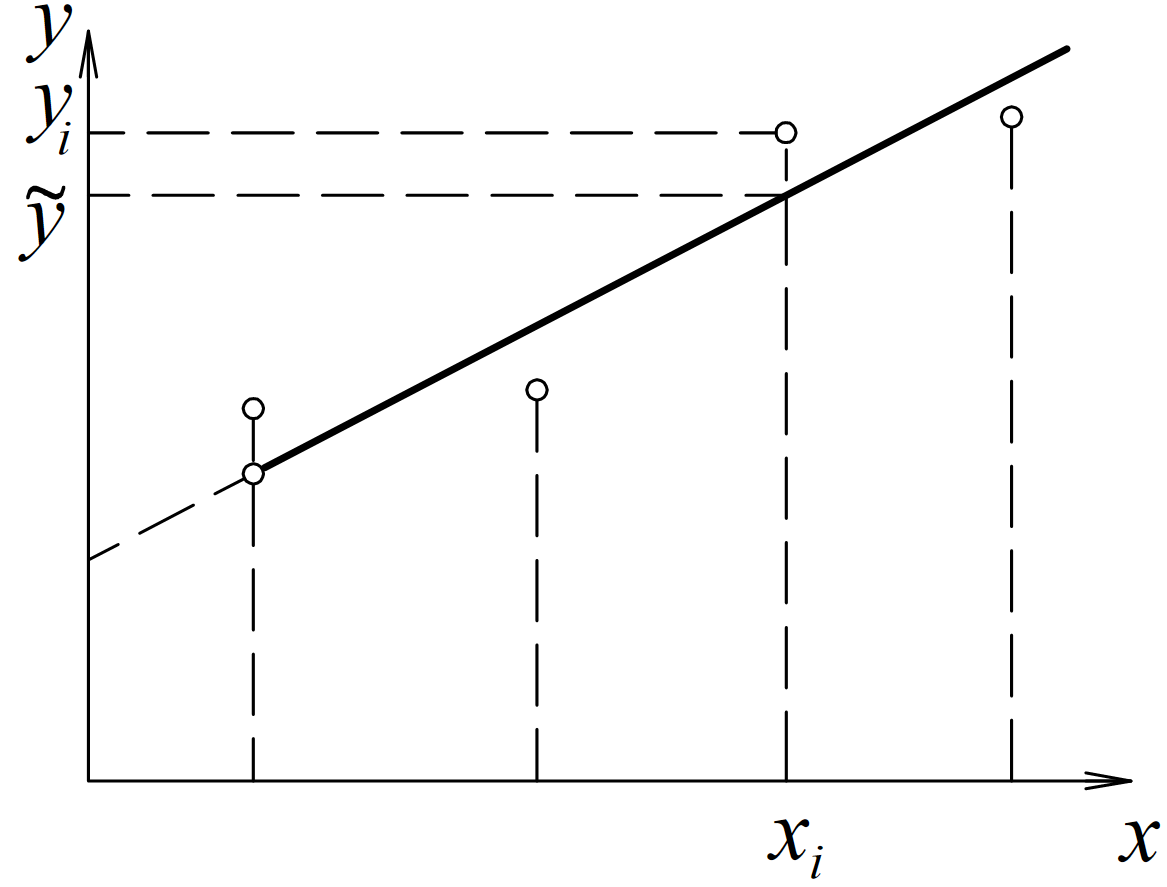
\includegraphics[width = 0.5\linewidth, keepaspectratio=true]{M11Addendum-LinearApproximation}
\end{center}
\caption{Линейная аппроксимация \label{fig:m11-linear-approx}}
\end{figure}

Для определения неизвестных параметров можно составить систему условных линейных уравнений, каждое из которых имеет вид: % интересно, что значит "условных"?
\begin{equation}
\label{eq:m11-linear-approx}
y_i = a x_i + b,\ i = 1, 2, \ldots, n. %не очень поняла, что такое К, поэтому убрала, и 3 убрала, потому что излишество, мб спец форматирование есть для этого
\end{equation}

Система уравнений~\eqref{eq:m11-linear-approx} при $n$-кратных измерениях может быть избыточной, если $n >2$ и, вообще говоря, несовместна, т.~к. результаты измерений величин $x$ и $y$ неизбежно содержат ошибки. Поэтому из этих уравнений можно определить лишь оценки $A$ и $B$ искомых параметров $a$, $b$, которые являются случайными величинами. %ИЗМ: ископаемых?!  -> искомых | почему A B стали вдруг большими? | допустим, я доросла и понимаю, почему они стали большими, надо только их поставить после "оценки", а не "параметров"

Будем считать, что все пары экспериментальных значений $x_i$, $y_i$  равновероятны (т.~е. измерения равноточные), случайные ошибки величин $x$ и $y$ распределены по нормальному закону, а систематическими ошибками можно пренебречь. Между рассчитанными по модели значениями $\widetilde{y_i}$ и экспериментальными отсчётами $y_i$ будут наблюдаться отклонения. Введём для них обозначения $\Delta_i = y_i - \widetilde{y_i} = y_i - (A  x_i + B)$. % "отсчетами"?
Математики Лежандр и Гаусс показали, что оценки $A$ и $B$ параметров $a$ и $b$  будут наиболее вероятными, если сумма квадратов отклонений по всем точкам $n$ будет наименьшей: %ИЗМ: "Лежнадр" -> "Лежандр" | мб "Лежандр и Гаусс" надо в запятые, хотя наверное нет ; вместо точки поставила двоеточие
\begin{equation}
\label{eq:m11-error}
Q = \isum \Delta_i^2 \to \min
\end{equation}

Минимум этой суммы находится по правилам дифференциального исчисления. Условием минимума функции является обращение в нуль частных производных функций $Q$ по независимым переменным $A$ и $B$:  % ИЗМ: разделила на 2 предложения
\begin{equation}
\label{eq:m11-derivative}
\frac{\partial Q}{\partial A} = 0; \ \frac{\partial Q}{\partial B} = 0. %;?!
\end{equation}

Подставляя~\eqref{eq:m11-error} в~\eqref{eq:m11-derivative}, получаем: %ИЗМ: "представляя" -> "подставляя"
\begin{equation}
\label{eq:m11-system}
\left\{ \aligned
&B \cdot \isum x_i + A \cdot \isum x_i^2 - \isum x_i y_i = 0 \\ % ИЗМ: "x_i \cdot y_i" -> "x_i y_i" вообще зачем столько cdot?
&A \cdot \isum x_i + n \cdot B - \isum y_i = 0  %убрала запятую и точку
\endaligned \right.
\end{equation}

Решая эту систему уравнений относительно параметров $A$ и $B$, находим: 
\begin{equation}
\label{eq:m11-solution}
\aligned
A &= \frac{n \cdot \isum x_i y_i - \isum x_i \cdot \isum y_i}{n \cdot \isum x_i^2 - \left( \isum x_i \right)^2}, \\
B &= \frac{\isum x_i^2 \cdot \isum y_i - \isum x_i \cdot \isum x_i y_i}{n \cdot \isum x_i^2 - \left( \isum x_i \right)^2}. %степень уехала
\endaligned
\end{equation}

Если разделить числители и знаменатели решений системы на $n^2$, то после несложных преобразований можно выразить коэффициенты $A$ и $B$ через средние значения величин, входящих в эти уравнения. Тогда получим: % ИЗМ: "уравнений системы (11.5)" -> "решений системы" 
\begin{equation}
\label{eq:m11-result}
\aligned
A &= \frac{\MTDMean{x  y} - \MTDMean{x} \cdot \MTDMean{y}}{\MTDMean{x^2} - \MTDMean{x}^2}, \\
B &= \frac{\MTDMean{x^2} \cdot \MTDMean{y} - \MTDMean{x} \cdot \MTDMean{x  y}}{\MTDMean{x^2} - \MTDMean{x}^2},
\endaligned
\end{equation}
где 
$
\MTDMean{x} = \frac{1}{n} \isum x_i, \ \MTDMean{y} = \frac{1}{n} \isum y_i, \ \MTDMean{x  y} = \frac{1}{n} \isum x_i y_i, \ \MTDMean{x} = \frac{1}{n} \isum x_i,\ \MTDMean{x^2} = \frac{1}{n}  \isum x_i^2
$
"--- средние арифметические значения соответствующих величин. Нахождение искомых оценок $A$ и $B$ по уравнениям~\eqref{eq:m11-result} удобно при ручном счете на микрокалькуляторах или на ЭВМ. 

Теория даёт возможность определить также дисперсию точек (рассеяние, отклонение экспериментальных точек от модельной прямой) и дисперсию коэффициентов $A$ и $B$. Если обозначить $S_0^2$ "--- дисперсию точек, $S_A^2$  и $S_B^2$  "--- дисперсии коэффициентов $A$ и $B$, то 
\begin{equation}
\label{eq:m11-S_0^2} % проверить формулы
S_0^2 = \frac{n}{n - 2} \cdot \left( \MTDMean{y^2} - \MTDMean{y}^2 - \frac{\left[ \hspace{3pt} \MTDMean{x y} - \MTDMean{x} \cdot \MTDMean{y} \hspace{3pt} \right] ^2}{\MTDMean{x^2} - \MTDMean{x}^2} \right), %все разной высоты
\end{equation}
\begin{equation}
\label{eq:m11-S_A^2}
S_A^2 =\frac{S_0^2}{n \cdot \left[ \hspace{3pt} \MTDMean{x^2} - \MTDMean{x}^2 \right]},
\end{equation}
\begin{equation}
\label{eq:m11-S_B^2}
S_B^2 = S_A^2 \cdot \MTDMean{x^2}.
\end{equation}

Интервалы, в которых с доверительной вероятностью $\beta$ могут находиться коэффициенты $a$ и $b$, записываются в виде
\begin{equation}
\label{eq:m11-range-1}
A - t_{\beta, n - 2} \cdot S_A \le a \le A + t_{\beta, n - 2} \cdot S_A,
\end{equation}
\begin{equation}
\label{eq:m11-range-2}
B - t_{\beta, n - 2} \cdot S_B \le b \le B + t_{\beta, n - 2} \cdot S_B,
\end{equation}
где $t_{\beta, n-2}$ "--- коэффициент Стьюдента. 

Полученные формулы непосредственно могут быть использованы для расчёта параметров линейных аппроксимирующих зависимостей в лабораторных работах. 


\end{document}
